\chapter{系统启动}
计算机上电后,系统会进行一系列初始化操作完成硬件设备的逐个启动。
早年这一个过程由执行每个设备上的ROM中存储的代码(一般称为固件firmware)结合BIOS完成。
随后,更加通用的UEFI被提出,UEFI的全称是Unified Extensible Firmware Interface,它是一套统一使用C语言编写在OS启动前的固件代码段。

\begin{figure}[h]
    \centering
    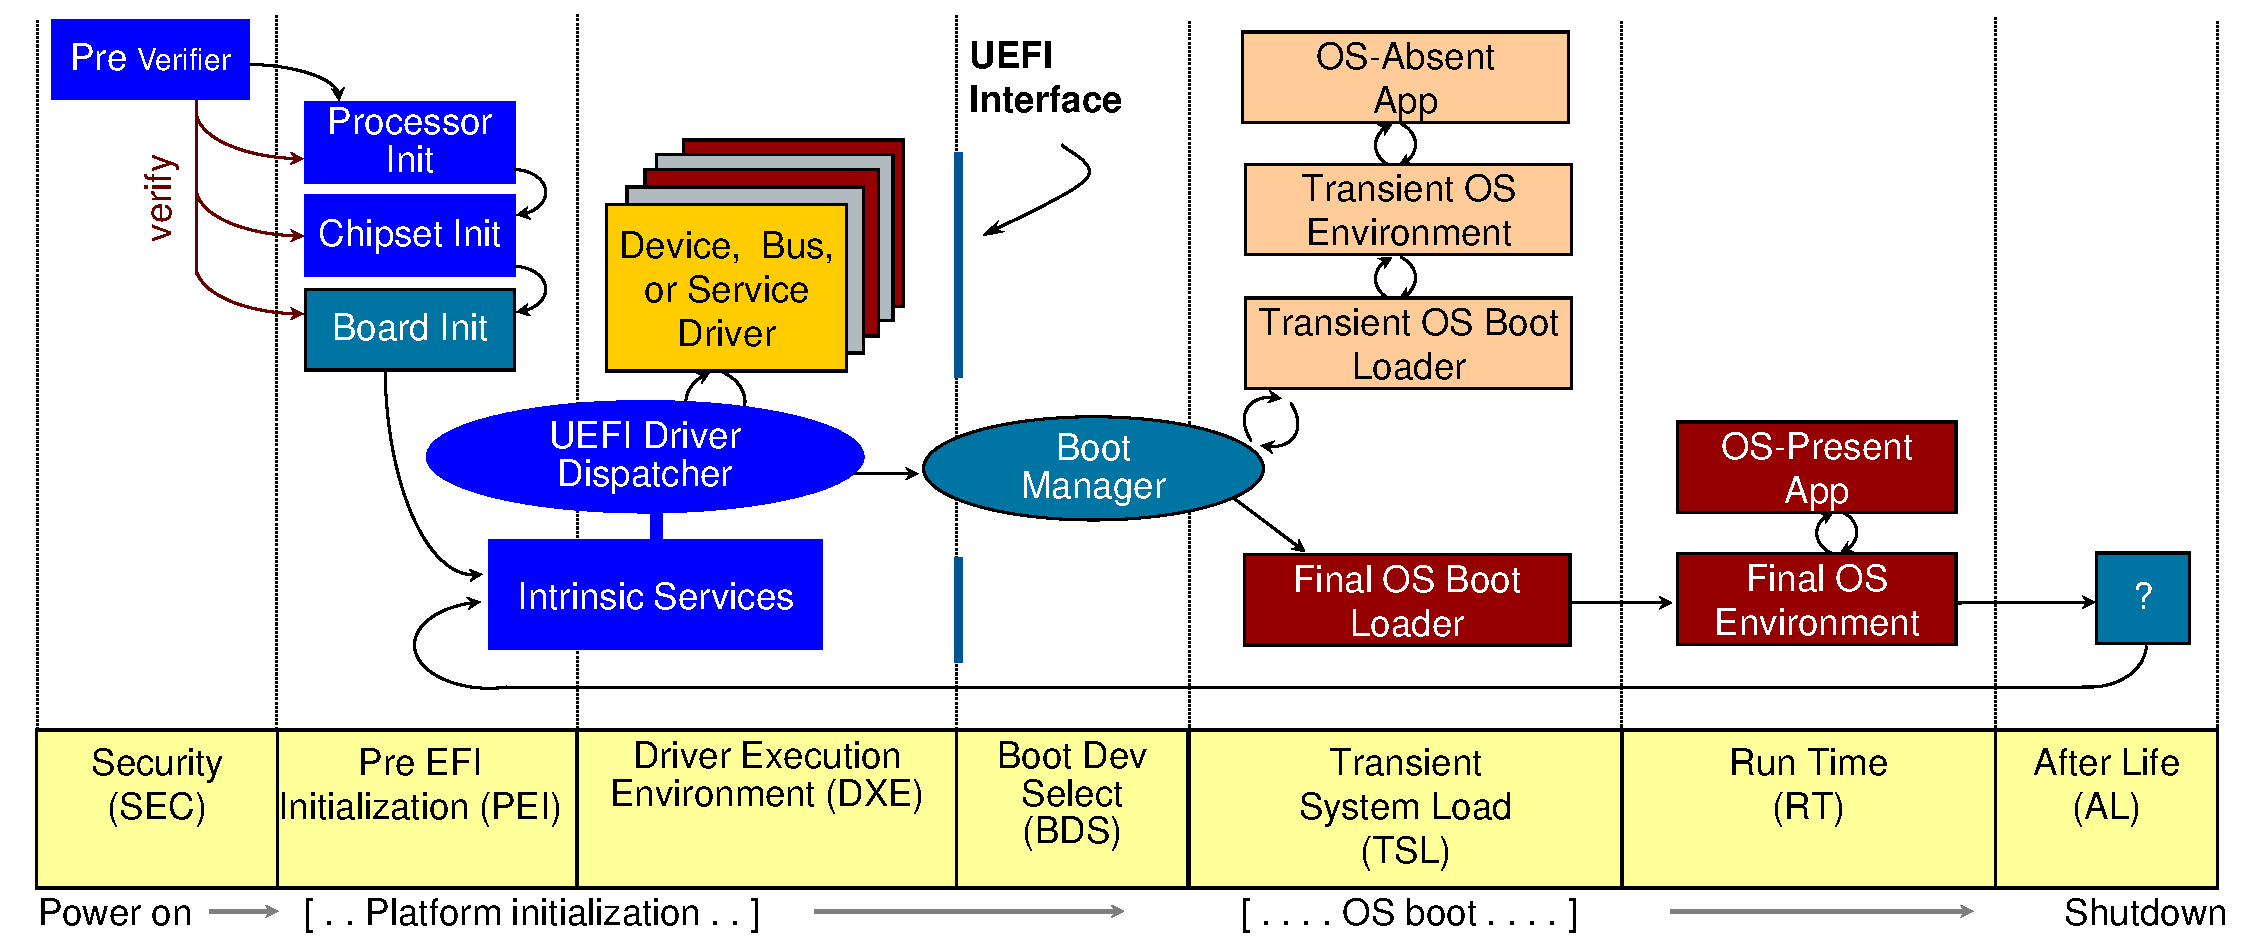
\includegraphics[width=\linewidth]{figure/mixed-figures/boot.pdf}
    \caption{UEFI启动过程}
    \label{fig:enter-label}
\end{figure}

这些固件代码段还会收集硬件信息,并且移交给操作系统。
早年的黑苹果、伪造OEM激活Windows 7都采用劫持UEFI启动后ACPI Table内容实现欺骗OS的效果。
在这个专题的实践中,我们需要体验读取、修改系统启动过程中的各个表,并且尝试传递更多的信息给操作系统。

\section{Read ACPI Table}
目标:修改EDK2的UEFI组件,在其中增加函数:\texttt{PrintAllACPITables}。该函数不传入任何参数,要求打印每一张表的地址、长度以及每一张其中所有的信息与校验信息。

可以参考EDK2下的\texttt{AcpiView.c} 中的 \texttt{AcpiView} 函数,但是不得直接复制。

此外,关于 ACPI 的更多信息,可以参考\href{https://uefi.org/sites/default/files/resources/ACPI_Spec_6.5a_Final.pdf}{这本手册}来学习,为了完成对应的任务,也许你只需要关注 ACPI 表的构成和 checksum 的含义即可。

具体测评指标:
\begin{itemize}
\item 输出所有ACPI表的完整地址映射;
\item 每个表的输出必须包含:物理地址(64位十六进制)、表长度(32位十进制)、OEM ID(6字节ASCII)、校验和(8位十六进制)。
\end{itemize}

\subsection{ACPI Table 结构}

ACPI Table 是一个树状结构,其第一张表是 RSDP(Root System Description Pointer),它里面存放了 RDST/XDST 的地址。RDST是32位地址,XDST是64位地址,其功能是一样的。
而 RDST/XDST 中记录了其他表的地址。

注意在 FADT(Fixed ACPI Description Table) 中有还记录 FACS 和 DSDT 的地址,这个两个表无法直接在 RDST/XDST 中找到。

\section{Hack ACPI Table}
目标:修改EDK2的UEFI组件,在其中增加函数:\texttt{ChangeACPITable}。该函数传入一个\texttt{UINTN}的对象表明修改第几张表、输入\texttt{EFI\_ACPI\_DESCRIPTION\_HEADER*}表明待修改的数值,要求修改完成后打印每一张表的地址、长度以及每一张其中所有的信息与校验信息。

测试:通过引导Linux后读取对应的ACPI表检查输出进行验证。

具体评测指标:
\begin{itemize}
\item 修改\texttt{EFI\_ACPI\_DESCRIPTION\_HEADER}中所有字段(包括Signature保留字段)且自动生成正确校验和的比例达到100\%;
\item 系统重启3次后修改仍然有效;
\item 内核日志(\texttt{dmesg | grep ACPI})无CHECKSUM\_ERROR警告或其他ACPI警告。
\end{itemize}

\section{UEFI运行时服务}
目标:增加一个新的UEFI运行时服务,使得Linux系统可以调用这个新的服务导出硬件运行时信息。

提示:需要修改UEFI固件和Linux内核(sysfs部分),方便直接读取导出的结果。

测试:展示
